\documentclass[ngerman,BCOR=4mm]{tudscrreprt}

% \usepackage[T1]{fontenc}
% fontspec ist für xelatex, fontenc für pdflatex
\usepackage[T1]{fontspec}
\usepackage[ngerman=ngerman]{hyphsubst}
\usepackage[ngerman]{babel}
\usepackage{isodate}
\usepackage[hidelinks]{hyperref}
\usepackage{amsmath, amsfonts, amssymb, amsthm} %% mathematics tools
\usepackage{csquotes}
\usepackage[draft]{listofsymbols}
\usepackage[backend=biber, urldateusetime=true, sorting=none]{biblatex} %% Literature citing engine
\usepackage{subcaption}

%__________Definitions_____________________________

% Literaturverzeichnis
\addbibresource{Literatur.bib}

% \newcommand{\bild}[2]{\includegraphics[width=#2\textwidth,height=#2\textheight,keepaspectratio]{#1}}
\newcommand{\bild}[4]{
      \begin{figure}[!htp]
            \centering
            \includegraphics[width=#2\textwidth,height=#2\textheight,keepaspectratio]{#1}
            \caption{#3}
            #4
      \end{figure}
}
\newcommand{\R}{\mathbb R}
\newcommand{\C}{\mathbb C}
\newcommand{\zitat}[1]{\glqq #1 \grqq}
\newcommand{\klammer}[1]{\left(#1\right)}
\newcommand{\AlamB}{A-\lambda\,B}

% wird für Symbolverzeichnis benutzt, sonst gibt es Fehler
\DeclareOldFontCommand{\bf}{\normalfont\bfseries}{\mathbf}


% Math
\theoremstyle{plain} % text is cursive
\newtheorem{theorem}{Theorem}
\newtheorem{lemma}[theorem]{Lemma}  %% [theorem] means same numbering for theorem and lemma
\newtheorem{proposition}[theorem]{Proposition}
\newtheorem{corollary}[theorem]{Korollar}

\theoremstyle{definition} % text is "upright"
\newtheorem{definition}[theorem]{Definition}
\newtheorem{example}[theorem]{Beispiel}

\theoremstyle{remark}
\newtheorem{remark}[theorem]{Bermerkung}

% Symbolverzeichnis
\renewcommand{\symheadingname}{Symbolverzeichnis}
\opensymdef
      % \newsym[]{}{}
      \newsym[Einheitsmatrix]{In}{I_n}
      \newsym[Massenmatrix]{M}{M}
      \newsym[Steifigkeitsmatrix]{K}{K}
      \newsym[Federkraft]{FL}{\overrightarrow{F_L}}
      \newsym[Trägheitskraft]{FT}{\overrightarrow{F_T}}
      \newsym[Verschiebung des k-ten Massepunktes aus der Ruhelage]{xk}{x_k}
      \newsym[Eigenkreisfrequenz]{w}{\omega}
\closesymdef


\begin{document}
\selectlanguage{ngerman}

%__________Deckblatt_Allg_Infos_____________________________
\faculty{Fakultät Mathematik}
\institute{Institut für Numerische Mathematik}
% \chair{Professur für Numerik partieller Differentialgleichungen}
\date{23.08.2024}
\title{%
      Gewichtete Eigenwert-Zählung auf einem Intervall
}
\subject{bachelor}
\graduation[B.Sc.]{Bachelor of Science}
\author{%
      Noah Göpel%
      \matriculationnumber{5029415}%
      \dateofbirth{01.02.2003}%
      \placeofbirth{Riesa}%
}
\matriculationyear{2021}
% \supervisor{}
\professor{Prof. Dr. Oliver Sander}
\maketitle

\clearpage
\tableofcontents
\clearpage
\listofsymbols
\clearpage

\chapter{Einleitung}
\label{sec: Einleitung}
      
      Diese Ausarbeitung beschäftigt sich mit numerischen Verfahren, um sicherzustellen, dass für ein gegebenes mechanisches System keine Eigenwerte in einem vorgegebenem festen Intervall liegen.
% hier muss noch einiges getan werden
      Damit kann sichergestellt werden, dass die Eigenfrequenzen des Systems nicht so liegen, dass es zu einer Selbsterregung kommt.

      % Um diese Anforderung zu erfüllen, werden die Eigenwerte des Matrix Pencils auf diesem Intervall gewichtet gezählt. Man erhält ein Minimierungsproblem,
      % in welchem es gilt, einen Design-Paramerter so anzupassen, dass auf dem Intervall kein Eigenwert des entsprechenden Systems mehr vorhanden ist.
      % Dazu werden in den Kapiteln \ref{sec: MS Matrizen} und \ref{sec: EW Problem} die theoretischen Grundlagen gelegt.
      % Anschließend werden in Kapitel \ref{sec: Quellen} die entscheidende Identität von Futamura und wichtige Überlegungen ausgeführt.

      % Daraufhin werden diese Überlegungen in Kapitel \ref{sec: Programmieren} anhand verschiedener Beispiele implementiert und getestet.

      Die Auswertung und Verbesserung der Implementation folgt in Kapitel \ref{sec: Verbesserungen}.

      % In dieser Ausarbeitung werden die gewichtete Zählung von Eigenwerten auf einem Intervall behandelt, um sicherzustellen,
      % dass bei einem vorgegebenem mechanischem System keine Eigenwerte in einem bestimmten festen Intervall liegen.
      % Dazu wird in den ersten Kapiteln die nötige Theorie anhand der Quellen \cite{grundlageFutamura} und \cite{hauptteilTkachuk} beschrieben.
      % Hier werden Matrix Pencil und das verallgemeinerte Eigenwertproblem verwendet, um 
      % Hierzu nutzt man die Identität von Futamura, um die Zählung der Eigenwerte auf die zugrundeliegenden Matrizen zurückzuführen.


      % und anschließend in Kapitel \ref{sec: Programmieren} in Python angewendet.
      % Daraufhin werden in Kapitel \ref{sec: Verbesserungen} die Ergebnisse kritisch betrachtet und weitere Algorithmen eingeführt, um die Berechnungen zu beschleunigen.
      Zum Schluss werden in Kapitel \ref{sec: Auswertung} die Ergebnisse wiederholt und ein Ausblick in weiterführende Themen gegeben.

      Ferner werden in Kapitel \ref{sec: Verbesserungen} eine Approximation der Matrix-Spur vorgestellt und ebenfalls implementiert.

\chapter{Das verallgemeinerte Eigenwert-Problem und die Identität von Futamura}
\label{sec: EW Problem_Futamura}

      Zu Beginn der Ausarbeitung werden einige Resultate über Matrizen und lineare Algebra behandelt.
      Diese werden in Kapitel \ref{sec: EW Zählung} verwendet, um die Zählung der Eigenwerte zu einer differenzierbaren Funktion umzustellen.
      
      \section{Der Matrix Pencil}
            Betrachte zunächst das Konzept des Matrix Pencil, welches in dieser Ausarbeitung eine entscheidende Rolle spielt.
            \begin{definition}(pencil, \cite[S. 375]{matrixGolub})
                  \label{def: pencil}
                  Seien $A$ und $B$ Matrizen in $\C^{n\times n}$, dann wird die Menge aller Matrizen der Form
                  $\AlamB, \lambda \in \C$ pencil genannt.
            \end{definition}

            Laut \cite[S. 375]{matrixGolub} seien die Eigenwerte von $\AlamB$ diejenigen $\lambda \in\C$, für die gelte:
            \begin{equation}
                  \label{eqn: verallg EW Problem}
                  (\AlamB)x=0,\quad x\ne 0
            \end{equation}
            
            Hier wird $x\in\C^n$ Eigenvektor genannt.
            Man beachte, dass für $B=\In$ Gleichung (\ref{eqn: verallg EW Problem}) die folgende Form annimmt:
            $$(A-\lambda\In)x=0 \Leftrightarrow Ax = \lambda x,$$
            also genau die Definition des Eigenwert-Problems.
% gibt es ein Eigenwert-Problem und wenn ja, gibt es eine Definition? oder ist es einfach eine Gleichung?
            Daher wird die Suche nach den $\lambda\in\C$, die (\ref{eqn: verallg EW Problem}) erfüllen auch verallgemeinertes Eigenwert-Problem genannt, da sie eine allgemeine Form des speziellen Eigenwertproblems darstellen.

            Falls man $\AlamB$ durch die Matrix $C$ ersetzt, so entsteht aus (\ref{eqn: verallg EW Problem}) das lineare homogene Gleichungssystem
            $$Cx=0,\quad x\ne 0$$

            Nach einem Resultat aus der linearen Algebra gilt:
% welches Resultat?, ich habe es bis jetzt nur in Skript LA20 gefunden
            $$\det(C)\ne 0 \Leftrightarrow Cx=0 \text{ hat als einzige Lösung }x=0$$
            Durch Negation folgt:
            $$\det(C)=0 \Leftrightarrow \exists x\ne 0: Cx=0$$

            Somit sucht man die Eigenwerte des Pencils, in dem man die Nullstellen des Polynoms $\det(\AlamB)$ berechnet\footnote{Man könnte das Polynom $\det(\AlamB)$ als eine Art charakteristisches Polynom des Pencils $\AlamB$ betrachten, ähnlich dem charakteristischen Polynom $f(A)$ einer Matrix $A$}.
            
            Daher wird in \cite[S. 375]{matrixGolub} die Menge der Eigenwerte des Pencils $\AlamB$ wie folgt definiert:
            \begin{equation}
                  \label{def: EW Pencil}
                  \lambda(A,B):=\{z\in\C:\ \det(A - zB) = 0\}
            \end{equation}

            Zum Schluss folgt noch eine Definition, welche in Kapitel \ref{sec: Futamura} benötigt wird:
            \begin{definition}
                  Ein Pencil heißt regulär, falls $B$ invertierbar ist.
            \end{definition}
% Quelle einfügen

            Man beachte, dass für einen regulären Pencil gilt:
            $$(\AlamB)x = 0 \Leftrightarrow (B^{-1}A - \lambda \In)x = 0$$
            Weshalb $$\lambda(A,B) = \lambda(B^{-1}A,\In) = \lambda(B^{-1}A),$$
            also kann man die Eigenwerte des regulären Pencils auf ein spezielles Eigenwertproblem zurückführen und die normalen Eigenwerte von $B^{-1}A$ sind genau die Eigenwerte des Pencils $\AlamB$.
      \section{Die Schur-Zerlegung}
      
      \section{Die Identität von Futamura}
      \label{sec: Futamura}
\chapter{Massen- und Steifigkeitsmatrizen}
\label{sec: MS Matrizen}
      Um die Eigenfrequenzen und/oder Eigenkreisfrequenzen \w eines Systems zu bestimmen, benötigt man zuerst die Massenmatrix \M und die Steifigkeitsmatrix \K des Systems.

      Laut \cite[S. 366]{maschinendynamikDresig} könne man für einfache Systeme das Prinzip von d'Alembert anwenden, es sei aber ungeeignet für komplexere Probleme.
            
      In diesem Kapitel werden 2 Systeme vorgestellt und die entsprechenden Matrizen berechnet:
      das erste ist ein Längsschwinger-System in einer Dimension, das zweite ein Längsschwinger in 2 Dimensionen.


% Erklärung x und anderes einfügen, auch Def Schwingersysteme
      Hier folgen nun Bilder, um die Systeme zu veranschaulichen:

      \begin{figure}[ht]
            \centering
            \begin{minipage}[ht]{0.49\linewidth}
                  \centering
                  \includegraphics[width=0.7\textwidth, keepaspectratio]{./src/Längsschwinger 1D.png}
                  \caption{Längsschwinger eindimensional}
                  \label{fig: Längsschwinger 1d}
            \end{minipage}
            \hfill
            \begin{minipage}[ht]{0.49\linewidth}
                  \centering
                  \includegraphics[width=0.7\textwidth, keepaspectratio]{./src/Längsschwinger 2D.png}
                  \caption{Längsschwinger zweidimensional}
                  \label{fig: Längsschwinger 2d}
            \end{minipage}
      \end{figure}

% in maschinendy gibt es def, was schwingersysteme sind 
      Hierbei haben die Federn keine Massen und es existieren weder Dämpfung noch Gewichtskraft.

      \section{Herleitung durch das Prinzip von d'Alembert}
            Nach \cite{d_AlembertPrinzip} besage das Prinzip von d'Alembert, dass die Summe aller wirkenden Kräfte in einem beschleunigten System verschwinde.

            Somit wird zuerst ein Kräftegleichgewicht aufgestellt und anschließend in Matrix-Schreibweise umgeformt, wodurch man die Massen- und Steifigkeitsmatrix erhält.
% In Maschinendynamik war von Koeffizientenvgl die Rede, könnte man auch einbauen
            Die erhaltene Gleichung muss die Form $M\,\ddot x+K\,x = 0$ besitzen. Dadurch können die gesuchten Matrizen an der Gleichung abgelesen werden.
% Es muss irgendwo eine Quelle geben, die genau das sagt
            Da diese Herleitung auf Kräftegleichgewichten beruht, werden nun die agierenden Kräfte kurz erläutert:

            Die Federkraft \FL wird laut \cite{federkraft} berechnet durch:
            \begin{equation}
                  \label{eqn: Federkraft}
                  \FL = -c\cdot \overrightarrow s,
            \end{equation}
            wobei $c$ die Federkonstante ist und $\overrightarrow s$ die Auslenkung der Feder aus der Ruhelage darstellt.

            Beachte, dass die Kraft entgegen der Auslenkung wirkt, da bei positiver Auslenkung die Feder sich zusammenziehen will, die Kraft also in die entgegengesetzte Richtung wirkt.
% Quelle finden
                  
            Die Trägheitskraft \FT ist definiert durch:
% Quelle
            \begin{equation}
                  \label{eqn: Trägheitskraft}
                  \FT = -m\cdot \overrightarrow{a}
            \end{equation}
            mit Masse $m$ und Beschleunigungsvektor $\overrightarrow{a}$.                  

            Um die Schematas klarer zu gestalten, werden die Kraftpfeile hier immer in die entgegengesetzte Richtung eingezeichnet, dafür aber die Minuszeichen weggelassen,
            somit werden in den Kraftschemas keine negativen Richtungen verwendet.
% Schemas, Kraftschemas, ...

            Generell sind $\FL,\ \overrightarrow{s},\ \FT \text{ und } \overrightarrow{a}\in \R^n$, aber in dieser Ausarbeitung werden sie immer als Skalare verwendet. 
            Da in diesem Kapitel Feder-Masse-Systeme behandelt werden, kann man $\overrightarrow{s}$ und $\overrightarrow{a}$ auf die Verschiebungen der Massen $(\xk)_k$ zurückführen:
            Im Allgemeinen wird hier $\overrightarrow{s}$ durch $(x_{k+1}-\xk)$ und $\overrightarrow{a}$ durch die zweite Ableitung $\ddot \xk$ ersetzt.
            Beide Kräfte werden in Abb. \ref{fig: KräfteAnFeder} veranschaulicht.

            \bild{./src/Federkraft und Trägheitskraft.png}{0.4}{wirkende Kräfte an Masse mit Feder \cite{federkraft}}{\label{fig: KräfteAnFeder}}
            
            In Abb. \ref{fig: KräfteAnFeder} ist $z$ die Auslenkung und $F_L$ ist als $c\cdot z$ definiert (vgl. \cite{federkraft}).
% Man könnte es auch umschreiben
            Betrachte nun einen Ausschnitt von Abb. \ref{fig: Längsschwinger 1d}: Die Massen $m_{k-1},\ m_k\text{ und }m_{k+1}$, wie es in Abb. \ref{fig: 3 Massen System} dargestellt wird.

            \begin{figure}[ht]
                  \centering
                  \begin{minipage}[ht]{0.49\linewidth}
                        \centering
                        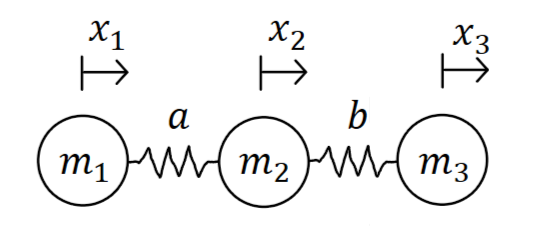
\includegraphics[width=0.7\textwidth, keepaspectratio]{./src/3 Massen System.png}
                        \caption{System mit 3 Massen}
                        \label{fig: 3 Massen System}
                  \end{minipage}
                  \hfill
                  \begin{minipage}[ht]{0.49\linewidth}
                        \centering
                        \includegraphics[width=0.7\textwidth, keepaspectratio]{./src/Kräfte Masse 1D.png}
                        \caption{Kräfte an frei geschnittener Masse}
                        \label{fig: Kräfte Masse 1D}
                  \end{minipage}
            \end{figure}

            Betrachtet man nur die $k$-te Masse, so erhält man die wirkenden Kräfte, wie sie in Abb. \ref{fig: Kräfte Masse 1D} dargestellt wurden.

            Mit dem Prinzip von d'Alembert führt dies auf die Gleichung
            \begin{equation}
                  \label{eqn: Gl für kte Masse}
                  m_k\,\ddot x_k + c_{k-1}\,(x_k-x_{k-1}) - c_k\,(x_{k+1}-x_k) = 0
            \end{equation}

            Man beachte, dass für unbewegliche Masse $m_{k-1}$, also für den Fall, dass
            $$x_{k-1} \equiv 0$$
            (\ref{eqn: Gl für kte Masse}) sich zu
            \begin{equation}
                  \label{eqn: Gl für kte Masse mit Rand links}
                  m_k\,\ddot x_k + c_{k-1}\,x_k - c_k\,(x_{k+1}-x_k) = m_k\,\ddot x_k + (c_{k-1}+c_k)\,x_k -c_k\,x_{k+1} = 0
            \end{equation}
            reduziert.

            In diesem Fall kann die $(k-1)$-te Masse als Rand betrachtet werden, für $k=1$ entspricht (\ref{eqn: Gl für kte Masse mit Rand links}) also genau der Gleichung für die Masse $m_1$ in Abb. \ref{fig: Längsschwinger 1d}.

            Falls man diese Gleichungen für alle n Massen aufstellt, dann können diese zu einer Gleichung der Art

            \begin{equation}
                  \label{eqn: MK Gleichung in 1D}
                  M\,\ddot x + K\,x = 0,\quad M,\ K\in\R^{n\times n}
            \end{equation}
            zusammengefasst werden. Anhand der gewonnenen Gleichung werden die Massen- und Steifigkeitsmatrix abgelesen.

            % Man sieht, dass hier M eine Diagonalmatrix ist, die nur positive Einträge auf der Hauptdiagonalen besitzt.
            % Sie ist somit insbesondere positiv definit, da alle Minoranten positiv sind.

            % Für den zwei-dimensionalen Fall benötigt man $n^2$ Punkt Massen und für jeden Punkt auch 2 Einträge in $x$, da es nun eine Bewegung in x- und in y-Richtung gibt.
            % Somit existieren $2\,n^2$ Einträge in $x$, aber jede Masse besitzt nur 2 Verbindungen mehr, somit wird die Steifigkeitsmatrix \K viel größer, aber auch viel schwächer besetzt.
            
      \section{Ermittlung der Matrizen der Modellprobleme}
            % Nun werden die Massen- und Steifigkeitsmatrix der obigen Systeme berechnet.
            Beginne dazu mit dem System aus Abb. \ref{fig: Längsschwinger 1d}

            Die Gleichung für $m_1$ ist durch (\ref{eqn: Gl für kte Masse mit Rand links}) mit $k=1$ gegeben.
            Für $k=2,\dots, n-1$ gilt (\ref{eqn: Gl für kte Masse}).
            
            Da die Masse $m_n$ durch die rechte Feder mit dem Rand verbunden ist, gilt analog zu oben $x_{n+1} \equiv 0$.
            Man erhält
            $$m_n\,\ddot x_n + c_{n-1}\,(x_n-x_{n-1}) + c_n\,x_n = 0.$$  

            Nach Umstellen folgt:
            \begin{equation}
                  \label{eqn: System GDgl MK 1d}
                  \begin{cases}
                        m_1\ \ddot x_1 + (c_0+c_1)\,x_1 - c_1\,x_2 & = 0   \\
                        m_i\ \ddot x_i - c_{i-1}\,x_{i-1} + (c_{i-1}+c_i)\,x_i -c_i\,x_{i+1} & = 0,\ i=2,...,n-1 \\
                        m_n\ \ddot x_n - c_{n-1}\,x_{n-1} + (c_{n-1}+c_n)\,x_n & = 0
                  \end{cases}
            \end{equation}

            Dieses System kann man zusammenfassen zu:
            $$M\,\ddot x + K\,x = 0,$$
            % damit wird die folgende Matrix quadratischer
            \renewcommand{\arraystretch}{1.5}
            wobei $$M= \text{diag}(m_1,\dots,m_n),\ 
            K = \begin{pmatrix}
                  c_0+c_1 & -c_1 &  &  & 0 \\
                  -c_1 & c_1+c_2 & -c_2 &  &  \\
                   & -c_2 & c_2+c_3 & \ddots &  \\
                    &  & \ddots & \ddots  & -c_{n-1} \\
                   0&  & & -c_{n-1} & c_{n-1}+c_n \\
                  \end{pmatrix}$$

                  
            % wird wieder auf Standard zurückgesetzt
            \renewcommand{\arraystretch}{1}
% Erklärung x? Oder kennt das jeder

% hier muss was über die Eigenschaften gesagt werden
            
            % Für das zwei-dimensionale System kann dieses Verfahren analog angewendet werden. 

      \section{Zusammenhang Eigenwert und Eigenfrequenz}
            Nach der Ermittlung der zugehörigen Matrizen, werden nun die Eigenfrequenzen des Systems bestimmt.
% Eigenkreisfrequenzen?

            Da in diesen Systemen die Massen um ihre Ruhelage schwingen und keine weiteren Kräfte wirken, schwingt jede einzelne Masse harmonisch.
            Nach \cite[S. 380]{maschinendynamikDresig} gilt daher mit $x$ statt $q$:
            $$x(t) = v\,\exp(i\w t),\ \ \ddot x(t) = -\w^2\,v \exp(i\w t)$$
            mit $v=(v_1,...,v_n)$ Vektor der Amplituden und der \zitat{noch unbekannten Eigenkreisfreqenz \w}\cite[S. 380]{maschinendynamikDresig}
            
            Diesen Ansatz kann man in (\ref{eqn: MK Gleichung in 1D}) einsetzen und erhält nach dividieren durch $\exp(i\w t)\footnote{offensichtlich ist die Division wohldefiniert, da $\exp(i\w t)\ne 0\ \forall \w, t\in\R,$}$:
            
            \begin{equation}
                  \label{eqn: verallg EW Problem mit w}
                  (K-\w^2\,M)\,v = 0
            \end{equation}

            Die Gleichung kann ebenfalls in \cite[S. 380]{maschinendynamikDresig} gefunden werden.

            Man will diese Gleichung für $v\ne 0$ lösen, da man sonst eine triviale Lösung erhält, in der keine Masse schwingt.


% braucht man wohl hier noch nicht
            Um (\ref{eqn: verallg EW Problem mit w}) mit $v\ne 0$ zu erfüllen, muss
            $$\det\klammer{K-\w^2\,M} = 0$$
            erfüllt sein.
% nachschlagen, warum das so ist

\chapter{Zählung von Eigenwerten}
\label{sec: EW Zählung}

      \section{Idee}
      \section{mathematische Formulierung}

\chapter{Implementierung}
\label{sec: Programmieren}
      \section{Erklärungen}

      \section{Implementation}

      \section{Grafiken}

\chapter{Verbesserungen}
\label{sec: Verbesserungen}
      \section{Auswertung bisheriger Implementation}

      \section{mögliche Verbesserungen}

      \section{Implementation und Auswertung der verbesserten Programme}

      \section{Approximation der Spur}

\chapter{Auswertung}
\label{sec: Auswertung}

\chapter{Literaturverzeichnis}

      % \begin{figure}[h]
      %       \centering
      %       \begin{minipage}[h]{0.49\linewidth}
      %       \centering
      %       \bilder{"./sources/himmel_und_wolken (www.umweltbundesamt.de)"}
      %       \caption{Betrachter:in auf der Erde}\cite{Himmel}
      %       \label{fig:himmel}
      %       \end{minipage}
      %       \hfill
      %       \begin{minipage}[h]{0.49\linewidth}
      %       \centering           
      %       \bilder{"./sources/erde (www.umweltbundesamt.de)"}
      %       \caption{Betrachter:in im Weltall auf die Erde}\cite{ErdeausWeltall}
      %       \label{fig:ErdeausWeltall}
      %       \end{minipage}
      % \end{figure}

      \printbibliography
\end{document}
